\documentclass{uebblatt}

\begin{document}

\maketitle{9}{}

\begin{aufgabe}{Simpliziale Mengen durch Erzeuger und Relationen}
\begin{enumerate}
\item Was ist die simpliziale Menge, die durch keinerlei Erzeuger erzeugt wird?
Was also ist das initiale Objekt in der Kategorie der simplizialen Mengen?
\item Was ist die simpliziale Menge, welche durch genau einen Erzeuger und
keine Relationen erzeugt wird?
\item Was ist die simpliziale Menge, die durch einen Erzeuger~$v \in X_1$ mit
der Relation~$d^0(v) = d^(v)$ erzeugt wird?
\end{enumerate}
\end{aufgabe}

\vfill
\centering
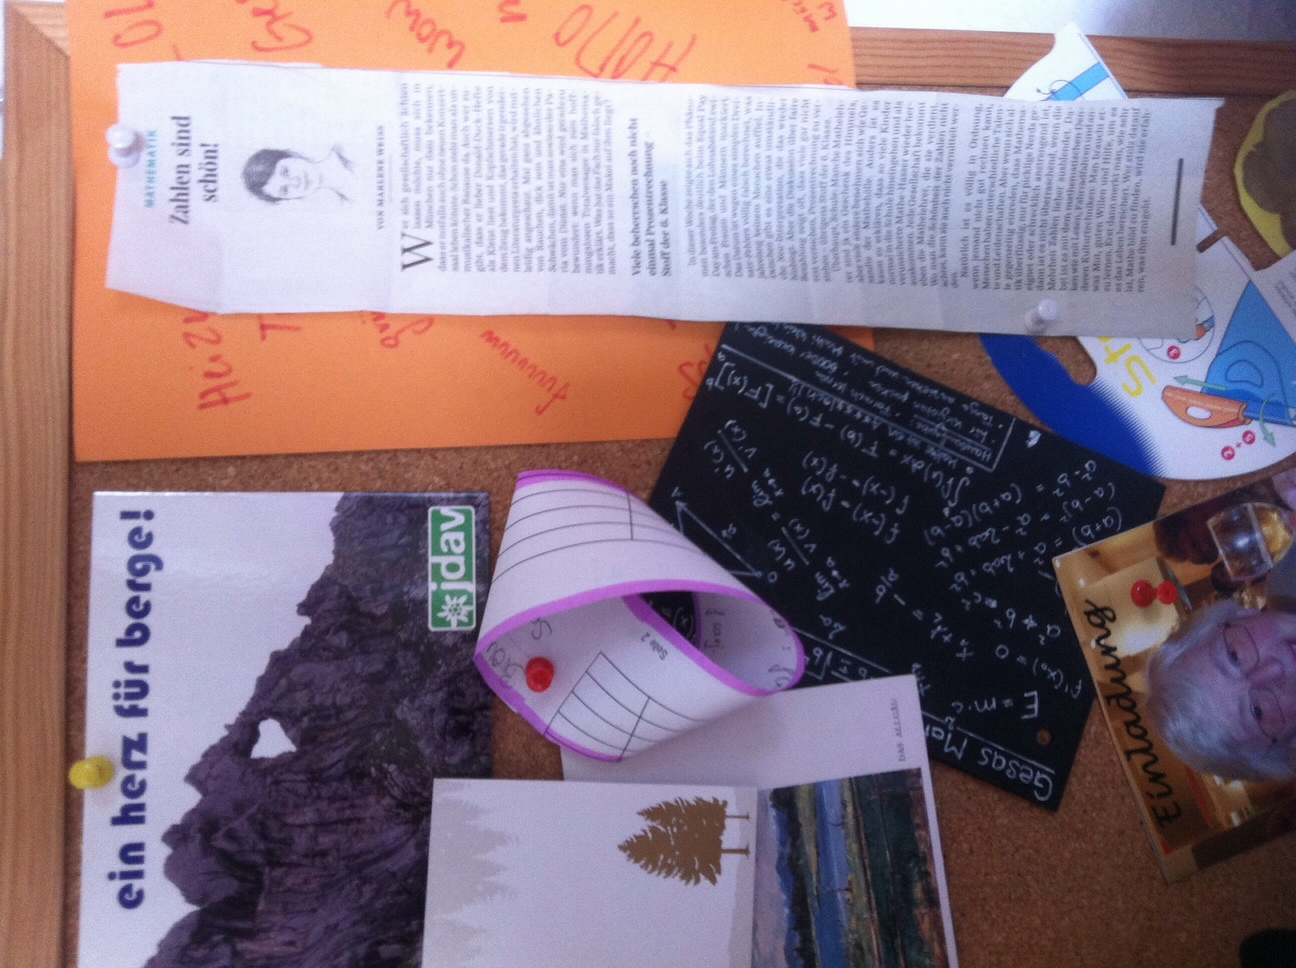
\includegraphics[scale=0.2]{images/moebiuspunkt}
\par

\end{document}
